\section{Вращательное движение твердого тела}
%TODO Ижевские олимпиады - вращательное движение

\begin{ex}
Определить ускорение тел и натяжение нити на машине Атвуда, предполагая, что $m_2>m_1$. Момент инерции блока относительно геометрический оси равен $I$, радиус блока $r$. Массу нити считать пренебрежимо малой. 
\begin{ans}
$a=g(m_1-m_2)/(m_1 +m_2 + I/r^2)$
\end{ans}
\end{ex}

\begin{ex}
\hspace{0pt} \\
\begin{minipage}{.65\textwidth}
(2010) На горизонтальной шероховатой поверхности лежит катушка ниток массой $m$. Ее момент инерции относительно собственной оси $I$, внешний радиус $R$, радиус намотанного слоя ниток $r$. Катушку без скольжения начали тянуть с постоянной силой $F$, направленной под углом $\alpha$ к горизонту. Найти ускорение центра катушки.
\end{minipage}
\begin{minipage}{.35\textwidth}
\centering
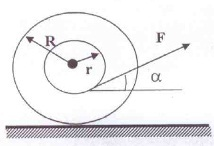
\includegraphics[width = 0.9\textwidth]{0717RotationDynamicsReelOfThread.jpg}
\end{minipage}
\begin{ans}
$a = F(\cos \alpha - r/R)/(m+I/R^2)$
\end{ans}
\end{ex}

%Сивухин-369
\begin{ex}
(2015) Гимнаст массы 80 кг, крутя солнышко на турнике. остановился и сделал стойку на руках (вверх ногами). Затем. немного отклонившись. начал вращаться, удерживая тело a прямом положении. Оценить максимальную силу натяжения, возникающую в каждой руке гимнаста.
\begin{ans}
$T=2mg$
\end{ans}
\end{ex}

%Сивухин-353
\begin{ex}
Монета массы $m$ и радиуса $r$, вращаясь в горизонтальной плоскости вокруг своей геометрической оси с угловой скоростью $\omega$, вертикально падает на горизонтальный диск и прилипает к нему. В результате диск приходит во вращение вокруг своей оси. Возникающий при этом момент сил трения в оси диска постоянен и равен $M_0$. Через какое время вращение диска прекратится? Сколько оборотов сделает диск до полной остановки? Момент инерции диска относительно его геометрической оси~$I_0$. Расстояние между осями диска и монеты равно~$d$.
\begin{ans}
$t=mr^2\omega/2M_0$, $N=M_0t^2/2I$, $I = I_0+m(d^2+r^2/2)$
\end{ans}
\end{ex}

\begin{ex}
Каким участком сабли следует рубить лозу, чтобы рука не чувствовала удар? Саблю считать однородной пластиной.
\begin{ans}
$l=2L/3$
\end{ans}
\end{ex}

%Сивухин-344
\begin{ex}
Сплошной однородный короткий цилиндр радиуса $R$, вращающийся вокруг своей геометрической оси со скоростью $\nu$ об/с, ставят в вертикальном положении на горизонтальную поверхность. Сколько оборотов $N$ сделает цилиндр, прежде чем вращение его полностью прекратится? Коэффициент трения скольжения между основанием цилиндра и поверхностью, на которую он поставлен, не зависит от скорости вращения и равен~$\mu$.
\begin{ans}
$N=3 \pi R \nu^2/(4\mu g)$
\end{ans}
\end{ex}

%Иродов-1.290
\begin{ex}
Однородный тонкий негнущийся стержень массой $m$ поддерживается в горизонтальном положении двумя вертикальными опорами у концов стержня. В начальный момент времени $t~=~0$ одна из опор выбивается. Найти силу, которая действует на вторую опору сразу же после этого момента.
\begin{center}
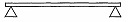
\includegraphics[width = 0.4\textwidth]{0705RotationDynamicsHorisontalBar.jpg}
\end{center}
\begin{ans}
$N = mg/4$
\end{ans}
\end{ex}

%Ижевск
\begin{ex}
\hspace{0pt} \\
\begin{minipage}{.65\textwidth}
Тонкий стержень массой $M$ и длиной $L$ свободно падает в вертикальной плоскости из начального положения, в котором угол между стержнем и горизонтальной плоскостью составлял $30^{\circ}$. Определите давление стержня на плоскость в момент удара, считая точку опоры стержня о плоскость неподвижной.
\end{minipage}
\begin{minipage}{.35\textwidth}
\centering
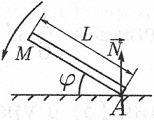
\includegraphics[width = 0.9\textwidth]{0709RotationDynamicsFallOfBar.jpg}
\end{minipage}
\begin{ans}
$N=\sqrt{10}Mg/4$
\end{ans}
\end{ex}

%Иродов-1.331
\begin{ex}
Сплошной цилиндр без проскальзывания катится со скоростью $v$ по горизонтальной плоскости, которая переходит в наклонную поверхность с углом $\alpha$. Радиус цилиндра $R$. Найти максимальное значение скорости цилиндра, при которой он перейдет на наклонную плоскость без скачка. Скольжения нет.
\begin{ans}
$v=\sqrt{gR(7\cos \alpha - 4)/3}$
\end{ans}
\end{ex}

\begin{ex}
(2003) Обруч радиуса $R$ бросают вперед со скоростью $v_0$ и сообщают ему одновременно угловую скорость $\omega_0$. 
Определить минимальное значение угловой скорости  $\omega_{0 \min}$, при котором обруч после движения с проскальзыванием покатится назад. 
Найти значение конечной скорости $v$, если $\omega_0 > \omega_{0 \min} $. Трением качения можно пренебречь.
\begin{ans}
$\omega_{0 \min} = v_0/R$, $v= (\omega_0R - v_0)/2$
\end{ans}
\end{ex}

%Сивухин-391
\begin{ex}
(2008) Сплошной однородный цилиндр, ось которого горизонтальна, движется без вращения по гладкой горизонтальной плоскости в направлении, перпендикулярном к его оси. В некоторый момент цилиндр достигает границы, где поверхность становится шероховатой и возникает постоянная (не зависящая от скорости) сила трения скольжения, а трение качения отсутствует. Каково будет движение цилиндра после перехода границы? Как распределится кинетическая энергия поступательного движения цилиндра?
\begin{sol}
Задача 391 сборника задач Сивухина.
\end{sol}
\begin{ans}
Движение после перехода границы будет сначала равнозамедленное, затем с постоянной скоростью; $1/3$ энергии превратится в тепло, $2/9$ во вращательную энергию и $4/9$ останется в виде поступательной энергии движения.
\end{ans}
\end{ex}

%----Закон сохранения момента импульса------
\begin{ex}
(2001) Пуля массы $m$, летящая горизонтально со скоростью $v$, попадает в покоящийся на шероховатой горизонтальной поверхности деревянный шар массой $M \gg m$  и радиусом $R$ на расстоянии $l$ ниже центра масс и застревает в нем. Найти установившуюся скорость шара.
\begin{ans}
$u = \frac{5mv}{7M}\left( 1 - l/R \right)$
\end{ans}
\end{ex}

%Иродов-1.310
\begin{ex}
(2004) Двум дискам радиусами $R_1$ и $R_2$ сообщили одну и ту же угловую скорость $\omega_0$, а затем их привели в соприкосновение, и система через некоторое время пришла в новое установившееся состояние движения. Оси дисков неподвижны, трения в осях нет. Моменты инерции относительно их осей вращения равны $I_1$ и $I_2$. Найти приращение момента импульса системы и приращение ее механической энергии.
\begin{ans}
$\Delta L = -4I_1I_2\omega_0/(I_1+I_2)$, $\Delta E = -2I_1I_2\omega_0^2/(I_1+I_2)$
\end{ans}
\end{ex}

%Сивухин-353
\begin{ex}
\hspace{0pt} \\
\begin{minipage}{.65\textwidth}
Тонкий стержень массы $m$ и длины $L$ подвешен за один конец и может вращаться без трения вокруг горизонтальной оси. К той же оси подвешен на нити дины $l$ шарик такой же массы $m$. Шарик отклоняют на некоторый угол и отпускают. При какой длине нити шарик после удара о стержень остановится? Удар абсолютно упругий.
\end{minipage}
\begin{minipage}{.35\textwidth}
\centering
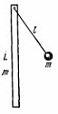
\includegraphics{0704RotationDynamicsBarAndBall.jpg}
\end{minipage}
\begin{ans}
$l = L/\sqrt{3}$
\end{ans}
\end{ex}

\begin{ex}
(2002) Шарик массой $m$ подвешен на нерастяжимой нити длиной $l$ и отклонен на малый угол от положения равновесия. В той же точке, что и нить, подвешен стержень длиной $1.5l$. Какова должна быть масса стержня $M$, чтобы в результате столкновения шарик остановился? Удар абсолютно упругий. Определить период колебаний шарика.
\begin{ans}
$M=2l/\sqrt{3}$, $T = 2\pi \sqrt{l/g}$
\end{ans}
\end{ex}

%Сивухин-408
\begin{ex}
(2007) На гладком горизонтальном столе лежит однородный твердый стержень длины $l$ и массы $M$, в край которого ударяет твердый шарик массы $m$, движущийся со скоростью $v_0$, перпендикулярной к оси стержня. Считая удар идеально упругим и предполагая, что силы трения между поверхностью стола и лежащими на ней телами пренебрежимо малы, вычислить угловую скорость вращения стержня после удара.
\begin{sol}
Решение задачи 408 сборника задач Сивухина.
\end{sol}
\begin{ans}
$\omega = \frac{12mv_0}{(4m+M)l}$
\end{ans}
\end{ex}

\begin{ex}
Шарик массой $m$ летит со скоростью $u_0$ навстречу покоящемуся стержню массой $M = 2m$ и длиной $2L$. Направление движения шарика перпендикулярно стержню и удалено на расстояние $l$ от его центра. После удара скорость шарика становится равной $u_1$, а стержня -- $V$. При этом стержень начинает вращаться с угловой скоростью $\omega$. Требуется определить 1) при каком $l$ шарик после удара остановится, а также 2) скорость шарика, стержня и угловую скорость вращения стержня, если шарик ударяет в конец стержня.
\begin{ans}
1) $l = L/\sqrt{3}$; 2) $u_1 = u_0/3$, $V=u_0/3$, $\omega = u_0/l$.
\end{ans}
\end{ex}

%Сивухин-397, Черепанов
\begin{ex}
Как надо ударить кием по бильярдному шару, чтобы при столкновении с другим (неподвижным) шаром 1) оба шара стали двигаться вперед (удар с накатом), 2) первый шар остановился, а второй двигался вперед (удар с остановкой), 3) второй шар двигался вперед, а первый откатился назад (удар с оттяжкой)? Предполагается, что удар наносится горизонтально в вертикальной плоскости, проходящей через центр шара и точку касания его с плоскостью бильярдного стола.
\begin{ans}
1) верхний удар $x > 2R/5$; 2) нормальный удар $x = 2R/5$; 3) нижний удар $x < 2R/5$.
\end{ans}
\end{ex}

%Черепанов - задача про игру в городки